%	 *** Licence ***
% Cette œuvre est diffusée sous les termes de la license Creative Commons
% «~CC BY-NC-SA 3.0~», ce qui signifie que :

% Vous êtes libres :

%   * de reproduire, distribuer et communiquer cette création au public ;
%   * de modifier cette création.

% Selon les conditions suivantes :
    	
%  * Paternité - vous devez citer le nom de l'auteur original de la manière indiquée par l'auteur de l'œuvre ou le
%	         titulaire des droits qui vous confère cette autorisation (mais pas d'une manière qui suggérerait
%	         qu'ils vous soutiennent ou approuvent votre utilisation de l'œuvre).
%  * Pas d’utilisation commerciale - Vous n'avez pas le droit d'utiliser cette œuvre à des fins commerciales. 
%  * Partage des conditions initiales à l'identique - si vous transformez ou modifiez cette œuvre pour en créer une nouvelle,
% 						      vous devez la distribuer selon les termes du même contrat ou avec une
%					              licence similaire ou compatible.

% Comprenant bien que :

%  * Renoncement - N'importe quelle condition ci-dessus peut être retirée si vous avez l'autorisation du détenteur des droits.
%  * Domaine public - Là où l'œuvre ou un quelconque de ses éléments est dans le domaine public selon le droit applicable, ce statut
%		      n'est en aucune façon affecté par le contrat.
%  * Autres droits - d'aucune façon ne sont affectés par le contrat les droits suivants :
%    - Vos droits de distribution honnête ou d’usage honnête ou autres exceptions et limitations au droit d’auteur applicables;
%    - Les droits moraux de l'auteur;
%    - Droits qu'autrui peut avoir soit sur l'œuvre elle-même soit sur la façon dont elle est utilisée, comme la publicité
%      ou les droits à la préservation de la vie privée.

% === Note ===

% Ceci est le résumé explicatif du Code Juridique; La version intégrale du contrat est consultable ici:
% <http://creativecommons.org/licenses/by-nc-sa/3.0/legalcode>.

\PoemTitle{À E.Khil (12 Septembre 2012)}
  \begin{lstlisting}
    #!/usr/bin/python2

    import random as troll
    gaga = troll.randint
    zero = 1

    while zero:
	  fun = gaga(1,42)
	  fun = (fun * "lo") + " "
	  print "Trolo" + fun

	  if not fun:
		  #FIXME: meaningless function
		  #troll.nyan(R,G,B)
		  break
    # KINGDOM  OF  HOLY ASS - RAINBOWED CATS
    # In case of incomprehension, break poetry and shit bricks
  \end{lstlisting}
  \paragraph{Note}
    Certains  font des  poèmes  à baisers,  nous  faisons nous  des
    poèmes à trolls.
    
    Il y en a 8 ici. Si  vous en voyez plus, vous êtes vous-même un
    troll.

\PoemTitle{LaTTrine (21 Septembre 2012)}
  \begin{center}
    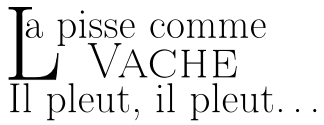
\includegraphics[scale=0.5]{emerge/lattrine.png}
  \end{center}

\PoemTitle{Jeu, 1 (26 Septembre 2012)}
  \begin{verse}
    Saint Etienne, martyr de son état\\
    homme qu’on abime à crocs de chiens\\
    ou sabots de lamas\\
    de courage se trouva bien dépourvu\\
    lorsque la pine du zèbre apparut!
  \end{verse}
  \begin{verse}
    «~Non, c’est assez, plutôt les ténèbres,\\
    les psaumes monocordes de sœur Emeline\\
    que cet enfer indigne qu’on le filme!~»
  \end{verse}

\PoemTitle{Jeu, 2 (26 Septembre 2012)}
  \begin{verse}
    Il est un jour où jamais\\
    l’excentrique cuistot ne rentre bredouille --\\
    le temps humide où l’escargot prend ses aises\\
    dans les recoins où la pluie mouille les fraises.
  \end{verse}
  \begin{verse}
    L’animal se balance, feuille à feuille,\\
    comme un écolier qui bave\\
    à son oral, dans une posture guère élégante
  \end{verse}
  \begin{verse}
    et \textsc{Paf}, s’abat soudain sur lui
  \end{verse}
  \begin{verse}
    \textsc{Quoi?}
    Une main.\\
    Tant pis pour toi, écolier,\\
    tant pis pour toi, escargot,
  \end{verse}
  \begin{verse}
    être dans les mâtinées grises\\
    incessement cuisiné\\
    c’était notre destin commun!
  \end{verse}
